
\section{Background research}

Penetration testing in general is a controlled form of hacking in which the tester acts as an attacker in order to find system misconfigurations and bugs that may lead to security threats {1}. There are generally two distinct approaches to penetration testing: White box and Black box. White box testing is also called structural testing because the test cases are designed based on the source code and are usually executed by software developers which are aware of internal code structure. Black box testing corresponds to functional testing and is intended to be performed without prior knowledge of the software internal mechanisms. The Black box pen testers focus on testing applications functionality and are only concerned about program input and output {2}. It has been noted that by combining these two methods it is possible to systematically discover target vulnerabilities and propose remediation {3}. It has further been proposed that penetration testing must not be regarded as the final stage before releases but become an integral part of the development cycle in order to prevent similar vulnerabilities from appearing in future applications {4}. 

There are numerous books written about penetration testing{5}, secure development cycles{x} and best practises regarding web applications{x}, embedded systems{x} and networking{x} but only a limited amount of information is available about IoT penetration testing specifically\cite{cookbook}. As later explained, IoT technologies just combine and modify previously developed solutions rather than inventing completely new technologies. The shift in use cases of well developed mechanisms and the amount of possible variations in the IoT environment requires a distinct look at it's security. That is one of the reasons why there is the need to adapt parts of classical infrastructure pen testing to rather distinct IoT field. Another important reason, is to make penetration testing less complicated for developers and people with less in-depth security related knowledge as well as create a convenience tool for existing penetration testers.

Although, there is no clear definition for the phrase Internet of Things, it is reasonable to define it as "the concept of every device blending with the existence of human beings"\cite{DBLP:journals/corr/MendezPY17}. Which means that smart devices mimic human interaction and other systems would not be able to distinguish a human interacting with it from another system. In it's simplest form IoT system definition can be rephrased as a decentralized network there multiple, usually, limited capabilities embedded processing units communicate between each other in various ways\cite{itu-t2060}. The fact that they have communication capabilities implies that they can change their behaviour depending on their network interface input and can essentially be controlled remotely. That is what exposes "smart objects" to outside threats\cite{riahi:hal-00868362}. Therefore, embedded system engineers, that were used to developing independent devices or small singular purpose closely bound networks, nowadays have to consider what consequences their decisions may have on the overall users infrastructure. Similarly the penetration testing complexity increases relative to the system size and technology set used. The addition of a network interface converts a narrow purpose device into an interactive Internet component.

Inserting a previously isolated technology into the global Internet network attracts malicious users attention. Unprotected log-ins, outdated software and insecure communication would not cause major security issues for hidden away, stand-alone embedded devices as long as they function properly (e.g. medical equipment). Situation changes drastically if a device can be discovered and interacted with by anyone on the network. Moreover, IoT devices can be extremely favourable targets for hackers that are expanding their bot nets. Unlike regular computers, IoT devices usually run continuously round-the-clock and can be exploited without owners knowledge\cite{191952}. It seems that traditional approaches of securing devices are not effective\cite{DBLP:journals/corr/abs-1803-05022} due to IoT technologies uniqueness and variety. Therefore, penetration testing is proposed as a way to imitate hacker attacks and evaluate IoT technologies security near to real world environment.

Above listed IoT inherited vulnerabilities require pen testing to be performed for every system layer, breaking down IoT network infrastructure and exposing hidden attack vectors. Testers must take into account 5 different aspects of IoT infrastructure. Hardware vulnerabilities can be exploited by anyone who has physical access to the device. Such vulnerabilities may be an open debugging port, password reset button and tapping into hardware level communication (e.g. UART)\cite{attify}. Firmware in this context stands for device operating system which can be rather primitive or extensive and may be using third party SDK and libraries that could introduce possible vulnerabilities\cite {cookbook}. Application level threats usually happen due to a software bug or a logic error\cite{cookbook}. If a device or an IoT system has a web interface, it essentially becomes a web host, thus it may have all the vulnerabilities of a regular website\cite{2007:WAH:1406550}. Communication and network exploits happen due to man-in-the-middle attacks and usage of insecure communication protocols assuming security by obscurity. Lastly, some IoT vendors release mobile applications complimenting their products. That is another new and troublesome attack vector as hackers may get access not only to victims IoT devices but also get a foot hold in users' smart phone and might be able to access personal information stored in there\cite{cookbook}. Only by addressing each part of the infrastructure individually and later as a whole one can thoroughly test an IoT system.



\subsection{Threat modelling}
According to the "IoT Penetration Testing Cookbook"\cite{cookbook} threat modelling can be broken down into these steps:
\begin{enumerate}
    \item Document all system assets using publicly available information: try to identify each device, write down all applicable information that may provide any hints on systems internal processes.
    \item Create architecture overview:
    \begin{itemize}
         \item Document IoT system functionality and features, create use cases
         \item Create architectural diagram that shows what components control flow
         \item Using architectural diagram and created use cases identify each individual component and communication method system communication method.
    \end{itemize}
    \item Use acquired system picture to identify entry points and write down possible threats. It does not have to be exact but it has to be backed up by some evidence.
    \item Starting with most likely threats determine:
    \begin{itemize}
        \item Threat targets 
        \item Possible exploitation techniques
        \item Possible countermeasures
    \end{itemize}
    \item Rate threats using DREAD rating system\cite{dread} and group them accordingly (High 12-15, Medium 8-11, Low 5-7)
    \item After the overall system analysis is finished, repeat the same process examining each part of the IoT system separately. Reuse previously created mapping and include new information reflecting on device specific threats. This is the time to logically and realistically evaluate each part of the system.
    Writing down possible threats for individual devices, mapping attack surfaces and identifying vulnerabilities which may lead to exploitation of distinct device weaknesses.
    \item Final step is to analyze and attack top ranking vulnerabilities of each system component (firmware, mobile application, communication, etc.) looking for a way in.
\end{enumerate}


\section{Project Goals}
This project goal is to collect information about IoT penetration testing and provide a tool that allows the generalized methodology to be easily applied in practise. The tool should be able to execute different types of network scans and display discovered devices in a user-friendly manner. The tool is also supposed to be able to apply information gathering techniques to individual devices such as port scanning. The idea is to visually present device and network specific information gathered from automatic and manual tests to get a better understanding of the system. By following penetration testing methodology it is then possible to identify attack surfaces and exposed entry points.

With initially gathered information a user can then choose one of the modular tools added to the application and apply device or protocol specific tests. The biggest advantage of a tool like this is its ability to use preexisting penetration tools to achieve individual tasks. As the IoT technology stack is so diverse it is impossible to design a tool that covers all the use cases. Instead, this project should provides a "tool box" which comes with a few basic testing tools and ability to add new tools if a need arises. The basic tools allow users to get a first view at the system of interest and make decisions about the next step.

As one of the emphasis of this application is to make IoT penetration testing more accessible and coherent for a diverse audience the ease-of-use and simplistic design are key aspects of the application. The whole tools functionality needs to be accessible via a graphical user interface with hints and explanations reducing the learning curve.

\subsection{Requirements}
    \subsubsection{Functional}
        \begin{itemize}
            \item Functionality to add and remove new security tools to and from the application
            \item Contain an initial proof-of-concept set of tools
            \item Scan local network, map network infrastructure and identify its components
            \item Support at least 2 communication protocols: WiFi and Bluetooth
            \item Provide guidelines and best practice for IoT penetration testing
            \item Give suggestions of most likely vulnerabilities in response to the initial network scan
            \item Allow chaining separate tool execution
            \item User is able to interact with the application via a graphical user interface
        \end{itemize}
    
    \subsubsection{Non-functional}
        \begin{itemize}
            \item Contains all required dependencies and is portable with little to no setup
            \item Compatible with most popular Linux distributions
            \item Must provide user with feedback within 2 second of user interaction
            \item Must be able to identify at least 25 unique devices on the network
        \end{itemize}

\subsection{Limitations}
This project cannot possibly find all existing IoT device vulnerabilities nor address specific firmware or hardware details; thus, it will only check for most frequent IoT device weak points. The tool set concentrates on finding application and communication level vulnerabilities. Some communication protocols may require special hardware tools and are harder to test. Because of the modular nature of the application design it may be possible to use such tools e.g. for capturing GSM communication packages \cite{DBLP:journals/corr/ShaikBANS15} but due to time and resource limitations it is out of scope of this module. It is also impossible to use the same technique to test an area as diverse as IoT networks. Therefore, the methodology provided is only guidelines gathered from multiple sources and may need alterations.

\subsection{Risk analysis}
Probability and Impact are rated in a scale from 1 to 5.

\def\riska{Loss of source code at some stage of development}
\def \probabilitya {1}
\def \impacta {4}
\def \mitigationa {Use of remote source control  repository to frequently record every stage of the development, thus being able to recover it if needed. }

\def\riskaa{Unable to fulfill all of the requirements due to technical implemention difficulties}
\def \probabilityaa {3}
\def \impactaa {2}
\def \mitigationaa {During the start of development process requirements will be split into tasks, divided into sprints and ranked using Agile methodology, therefore ensuring that core functionality will be implemented first and a working proof of concept is available at the end of the project }

\def\riskaaa{Loss of development time due to other course modules}
\def \probabilityaaa {2}
\def \impactaaa {2}
\def \mitigationaaa {Dedicate fixed amount of time every week for the project in order to keep up with the schedule }

\def\riskaaaa{Some part of the project taking up significantly longer that expected}
\def \probabilityaaaa {3}
\def \impactaaaa {2}
\def \mitigationaaaa {Re-evaluate task importance and readjust development schedule in order to deliver functional prototype }

\def\riskaaaaa{Unable to complete adequate application testing due to technical or time limitations}
\def \probabilityaaaaa {3}
\def \impactaaaaa {3}
\def \mitigationaaaaa {Complete limited or partial testing concentrating on core functionality, document causes and reasoning. If difficulties arise in early stages of development  due to technical limitations, seek support from university staff that have more experience in similar situations. }

\begin{center}
\begin{tabular}{ |m{5cm}|m{2cm}|m{1cm}|m{6cm}| } 
 \hline
 Risk & Probably & Impact & Mitigation \\ 
 \hline
 \riska & \probabilitya & \impacta & \mitigationa \\ 
 \hline
 \riskaa & \probabilityaa & \impactaa & \mitigationaa \\ 
 \hline
 \riskaaa & \probabilityaaa & \impactaaa & \mitigationaaa \\ 
 \hline
 \riskaaaa & \probabilityaaaa & \impactaaaa & \mitigationaaaa \\ 
 \hline
 \riskaaaaa & \probabilityaaaaa & \impactaaaaa & \mitigationaaaaa \\ 
 \hline
\end{tabular}
\end{center}



\section{Application design}
The penetration testing tool is chosen to be a desktop based GUI application. Desktop applications will have no dependencies on browsers. Server side - client side code complications and JavaScript engine dependencies are also removed. It is planned that all libraries and resources required for the application to run would be included in the final deliverable, thus increasing portability and reducing setup complexity. Additional features as automatic update service and application error scan is planned in order to keep software up to date by using git repository as a code base.

Application will implement modular design to re-use existing penetration tools and follow usage-centered design principles. In order to add a tool to the tool set, a user will have to define an interface/wrapper for the new tool. The wrapper will contain instructions on how to convert GUI input to tool specific commands as well as interpret tools output. This design allows flexibility and makes no assumptions about individual tool input or output. By prioritizing usability and clarity the application will remain user friendly and minimize new users learning curve \cite{user}.

It has been decided that the application will be written in Python. Python is a dynamic scripting language suitable for rapid development and prototyping. There will be no learning curve to use it as work experience is already present. Graphic User Interface will be developed using PyQT library as it is highly customize and popular between Python developers. Python is also by default present in the majority of Linux distributions, therefore no additional setup will be required. Other alternatives as Java, JavaScript and C++ were considered but were dismissed due slower development cycle, steeper learning curve or lack. One may point out Python lesser performance as a disadvantage but as the majority of computationally heavy tasks will be executed by other tools that does not make any difference.

A UML diagram present describes general application structure.

\begin{figure}[h!]
\caption{UML diagram}
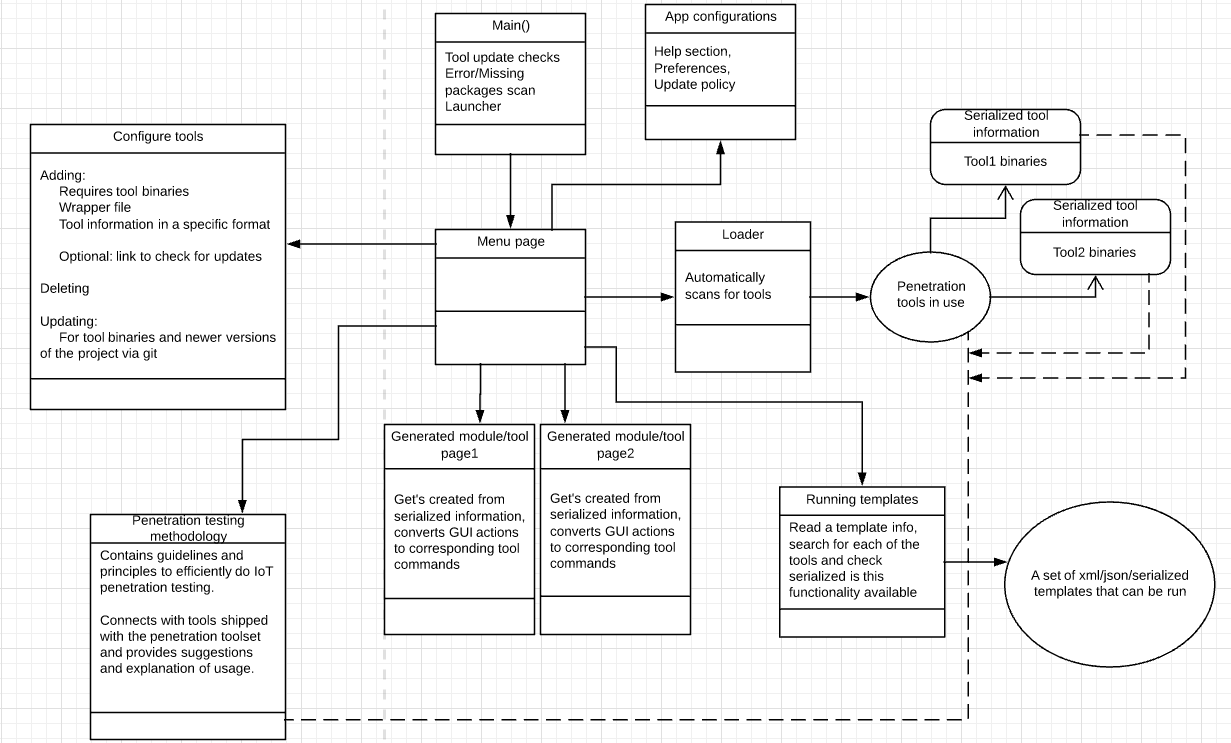
\includegraphics[width=\linewidth]{UML-diagram}
\centering
\end{figure}

\section{Remaining work}

Work completed up to this point and the remaining work is visualized using Gannt chart. The application design and background research phases are completed. The remaining development time will be mostly divided into sprints of 10-14 days in order to assign time for inevitable other module assignments. Each sprint will have a predefined set of tasks prioritized in Agile manner. After the sprint is completed planned functionality is supposed to be fully functional and tested to constantly add value. The Christmas period, January exam period and Easter periods are planned in looser manner in order to accommodate vacations, assess progress and re-think design decisions. The last weeks of the project are reserved for writing final report.

\begin{figure}
\caption{Gannt chart}
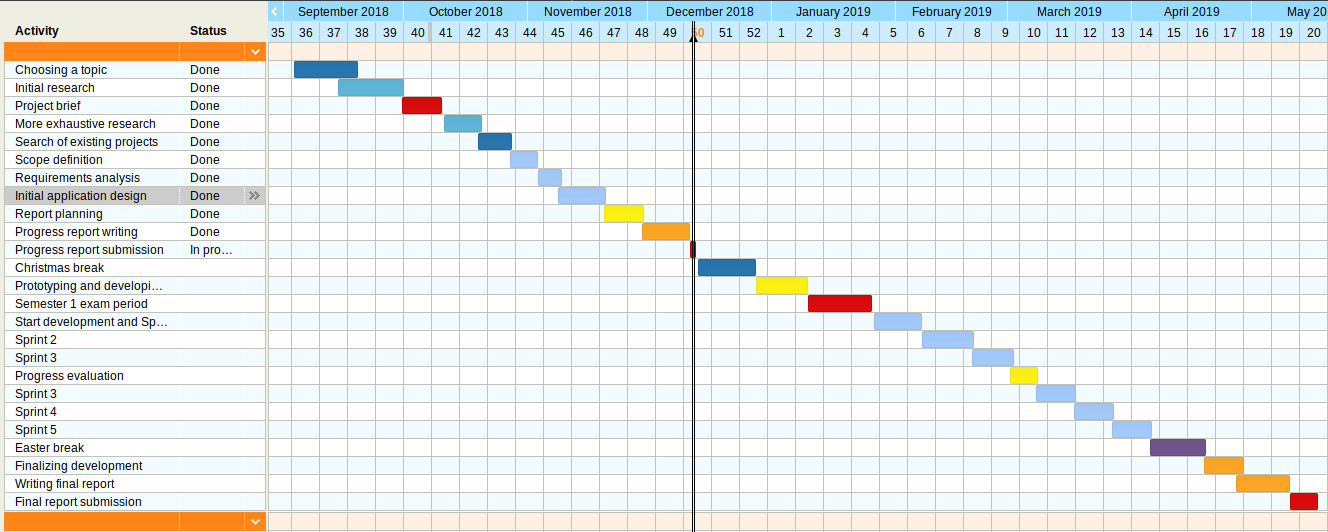
\includegraphics[width=\linewidth]{Gannt}
\centering
\end{figure}